\documentclass[14pt,dvipdfmx,uplatex]{beamer}
\usetheme{Madrid}
\usepackage{pxjahyper}
\setbeamertemplate{footline}[page number]{}
\setbeamercovered{transparent=35}
\beamertemplatenavigationsymbolsempty
\usepackage{mypresentation}
\usepackage{minted}
\usepackage{fvextra}
\usepackage{lucidabr}
\usepackage{multicol}
%\AtBeginShipoutFirst{\special{pdf:tounicode EUC-UCS2}}
\usepackage{tikz}
\usepackage[breakable, skins]{tcolorbox}
\usetikzlibrary{arrows}
\usetikzlibrary{shapes.callouts}
\usetikzlibrary{decorations.pathmorphing}
\usetikzlibrary{positioning}

\usepackage[noalphabet]{pxchfon}
\definecolor{ikkonzome}{rgb}	{	0.9961	,	0.7569	,	0.7373	}
\definecolor{ishitake}{rgb}	{	0.9961	,	0.6941	,	0.7059	}
\definecolor{momo}{rgb}	        {	0.9961	,	0.6824	,	0.8039	}
\definecolor{kobai}{rgb}	{	0.9412	,	0.4235	,	0.5569	}
\definecolor{nakabeni}{rgb}	{	0.9451	,	0.2706	,	0.4941	}
\definecolor{sakura}{rgb}	{	0.9333	,	0.8353	,	0.8353	}
\definecolor{arazome}{rgb}	{	0.9725	,	0.7216	,	0.7843	}
\definecolor{usubeni}{rgb}	{	0.8471	,	0.4471	,	0.5451	}
\definecolor{hisame}{rgb}	{	0.7451	,	0.4039	,	0.4039	}
\definecolor{toki}{rgb}	        {	0.9569	,	0.6431	,	0.6353	}
\definecolor{sakuranezumi}{rgb}	{	0.6941	,	0.6039	,	0.6078	}
\definecolor{sango}	{rgb}	{	0.8471	,	0.4157	,	0.3725	}
\definecolor{akane}	{rgb}	{	0.7529	,	0.0118	,	0.3451	}
\definecolor{choshun}{rgb}	{	0.7490	,	0.5255	,	0.5255	}
\definecolor{karakurenai}{rgb}	{	0.7373	,	0.0118	,	0.2667	}
\definecolor{enji}{rgb}	        {	0.6275	,	0.0863	,	0.3176	}
\definecolor{keshiaka}{rgb}	{	0.6275	,	0.4275	,	0.4275	}
\definecolor{kokiake}{rgb}	{	0.5059	,	0.0706	,	0.2549	}
\definecolor{jinzamomi}{rgb}	{	0.9098	,	0.4549	,	0.4157	}
\definecolor{mizugaki}{rgb}	{	0.7294	,	0.5529	,	0.4784	}
\definecolor{umenezumi}{rgb}	{	0.5882	,	0.3922	,	0.3882	}
\definecolor{suoko}{rgb}        {	0.5843	,	0.2667	,	0.2431	}
\definecolor{akabeni}{rgb}	{	0.8039	,	0.0784	,	0.3725	}
\definecolor{shinshu}{rgb}	{	0.6431	,	0.0353	,	0.0000	}
\definecolor{azuki}{rgb}	{	0.5255	,	0.0235	,	0.0000	}
\definecolor{ginshu}{rgb}	{	0.7490	,	0.2824	,	0.0588	}
\definecolor{ebicha}{rgb}	{	0.4549	,	0.2706	,	0.2627	}
\definecolor{kuriume}{rgb}	{	0.5843	,	0.3804	,	0.4314	}
\definecolor{akebono}{rgb}	{	0.8902	,	0.5961	,	0.4941	}
\definecolor{hanezu}{rgb}	{	0.7882	,	0.5961	,	0.5373	}
\definecolor{sangoshu}{rgb}	{	0.8196	,	0.5059	,	0.4471	}
\definecolor{shozyohi}{rgb}	{	0.7686	,	0.0000	,	0.0000	}
\definecolor{shikancha}{rgb}	{	0.5569	,	0.3294	,	0.1882	}
\definecolor{kakishibu}{rgb}	{	0.6745	,	0.4078	,	0.3333	}
\definecolor{benikaba}{rgb}	{	0.7137	,	0.3373	,	0.2941	}
\definecolor{benitobi}{rgb}	{	0.6196	,	0.3176	,	0.2706	}
\definecolor{benihihada}{rgb}	{	0.5020	,	0.3137	,	0.2353	}
\definecolor{kurotobi}{rgb}	{	0.3176	,	0.2000	,	0.1490	}
\definecolor{benihi}{rgb}	{	0.8235	,	0.4745	,	0.1922	}
\definecolor{terigaki}{rgb}	{	0.8118	,	0.4627	,	0.1804	}
\definecolor{ake}{rgb}	        {	0.7804	,	0.3098	,	0.1725	}
\definecolor{edocha}{rgb}	{	0.6863	,	0.4353	,	0.2941	}
\definecolor{bengara}{rgb}	{	0.6392	,	0.1569	,	0.0196	}
\definecolor{hihada}{rgb}	{	0.5412	,	0.3412	,	0.2353	}
\definecolor{shishi}{rgb}	{	0.8549	,	0.6863	,	0.5961	}
\definecolor{araishu}{rgb}	{	0.9294	,	0.4902	,	0.4549	}
\definecolor{akago}{rgb}	{	0.8118	,	0.5765	,	0.4275	}
\definecolor{tokigaracha}{rgb}	{	0.7922	,	0.5255	,	0.3686	}
\definecolor{otan}{rgb}	        {	0.8157	,	0.4157	,	0.2235	}
\definecolor{komugi}{rgb}	{	0.8157	,	0.6549	,	0.5098	}
\definecolor{rakuda}{rgb}	{	0.6784	,	0.5255	,	0.4118	}
\definecolor{tsurubami}{rgb}	{	0.6275	,	0.4392	,	0.3961	}
\definecolor{ama}{rgb}	        {	0.7765	,	0.6902	,	0.5843	}
\definecolor{nikkei}{rgb}	{	0.7216	,	0.4667	,	0.3725	}
\definecolor{renga}{rgb}	{	0.6902	,	0.3765	,	0.3098	}
\definecolor{sohi}{rgb}   	{	0.8078	,	0.5098	,	0.2078	}
\definecolor{enshucha}{rgb}	{	0.6706	,	0.4275	,	0.1608	}
\definecolor{karacha}{rgb}	{	0.5765	,	0.4235	,	0.1490	}
\definecolor{kabacha}{rgb}	{	0.6353	,	0.3725	,	0.1569	}
\definecolor{sodenkaracha}{rgb}	{	0.5216	,	0.3490	,	0.1373	}
\definecolor{suzumecha}{rgb}	{	0.4745	,	0.3176	,	0.1255	}
\definecolor{kurikawacha}{rgb}	{	0.4078	,	0.2745	,	0.1098	}
\definecolor{momoshiocha}{rgb}	{	0.3490	,	0.2353	,	0.0902	}
\definecolor{tobi}{rgb}	        {	0.4353	,	0.3098	,	0.1412	}
\definecolor{kurumizome}{rgb}	{	0.6667	,	0.5333	,	0.3333	}
\definecolor{kaba}{rgb}	        {	0.8196	,	0.4588	,	0.1294	}
\definecolor{korosen}{rgb}	{	0.5059	,	0.3843	,	0.1608	}
\definecolor{kogecha}{rgb}	{	0.3333	,	0.2549	,	0.1098	}
\definecolor{kokikuchinashi}{rgb}	{	0.8078	,	0.5922	,	0.3490	}
\definecolor{araigaki}{rgb}	{	0.8157	,	0.5529	,	0.3176	}
\definecolor{taisha}{rgb}	{	0.6353	,	0.4196	,	0.2078	}
\definecolor{akashirotsurubami}{rgb}	{	0.8078	,	0.6118	,	0.4157	}
\definecolor{tonocha}{rgb}	{	0.5922	,	0.4039	,	0.2000	}
\definecolor{sencha}{rgb}	{	0.5255	,	0.3529	,	0.1490	}
\definecolor{sharegaki}{rgb}	{	0.8549	,	0.7098	,	0.4863	}
\definecolor{ko}{rgb}	        {	0.9529	,	0.8275	,	0.6627	}
\definecolor{usugaki}{rgb}	{	0.8627	,	0.7294	,	0.5294	}
\definecolor{koji}{rgb}	        {	0.8275	,	0.6039	,	0.2706	}
\definecolor{umezome}{rgb}	{	0.8667	,	0.7373	,	0.4235	}
\definecolor{beniukon}{rgb}	{	0.8549	,	0.5843	,	0.2549	}
\definecolor{chojicha}{rgb}	{	0.5569	,	0.4000	,	0.1098	}
\definecolor{kenpozome}{rgb}	{	0.3059	,	0.2667	,	0.0627	}
\definecolor{biwacha}{rgb}	{	0.7333	,	0.5294	,	0.1922	}
\definecolor{kohaku}{rgb}	{	0.8039	,	0.5961	,	0.2471	}
\definecolor{usuko}{rgb}	{	0.8745	,	0.7373	,	0.4824	}
\definecolor{kuchiba}{rgb}	{	0.8157	,	0.6157	,	0.3216	}
\definecolor{kincha}{rgb}	{	0.7725	,	0.4902	,	0.2000	}
\definecolor{chozizome}{rgb}	{	0.5686	,	0.3961	,	0.1608	}
\definecolor{kitsune}{rgb}	{	0.6392	,	0.4431	,	0.1804	}
\definecolor{hushizome}{rgb}	{	0.5804	,	0.4353	,	0.1608	}
\definecolor{kyara}{rgb}	{	0.4510	,	0.3373	,	0.1255	}
\definecolor{susutake}{rgb}	{	0.4588	,	0.3529	,	0.1176	}
\definecolor{shirocha}{rgb}	{	0.7529	,	0.6588	,	0.4118	}
\definecolor{odo}{rgb}	        {	0.7137	,	0.6039	,	0.3137	}
\definecolor{ginsusutake}{rgb}	{	0.5608	,	0.4745	,	0.2392	}
\definecolor{kigaracha}{rgb}	{	0.7490	,	0.6196	,	0.2745	}
\definecolor{kobicha}	{rgb}	{	0.5020	,	0.4118	,	0.1765	}
\definecolor{usuki}	{rgb}	{	0.8549	,	0.7804	,	0.4275	}
\definecolor{yamabuki}	{rgb}	{	0.9098	,	0.8000	,	0.2039	}
\definecolor{tamago}	{rgb}	{	0.8275	,	0.7412	,	0.3373	}
\definecolor{hajizome}	{rgb}	{	0.7412	,	0.6039	,	0.2431	}
\definecolor{yamabukicha}{rgb}	{	0.7059	,	0.5765	,	0.2275	}
\definecolor{kuwazome}	{rgb}	{	0.6471	,	0.5255	,	0.2118	}
\definecolor{namakabe}	{rgb}	{	0.5569	,	0.4549	,	0.1843	}
\definecolor{kuchinashi}{rgb}	{	0.8078	,	0.7333	,	0.3843	}
\definecolor{tomorokoshi}{rgb}	{	0.7804	,	0.7020	,	0.2941	}
\definecolor{shirotsurubami}{rgb}	{	0.8745	,	0.8235	,	0.5922	}
\definecolor{kitsurubami}{rgb}	{	0.6863	,	0.6039	,	0.2118	}
\definecolor{toou}	{rgb}	{	0.8353	,	0.7725	,	0.4235	}
\definecolor{hanaba}	{rgb}	{	0.8549	,	0.8000	,	0.4941	}
\definecolor{torinoko}	{rgb}	{	0.8431	,	0.8118	,	0.6902	}
\definecolor{ukon}	{rgb}	{	0.8039	,	0.7216	,	0.3059	}
\definecolor{kikuchiba}	{rgb}	{	0.7765	,	0.6667	,	0.2902	}
\definecolor{rikyushiracha}{rgb}{	0.6627	,	0.6471	,	0.4784	}
\definecolor{rikyucha}	{rgb}	{	0.5176	,	0.5176	,	0.2588	}
\definecolor{aku}	{rgb}	{	0.5294	,	0.5059	,	0.4039	}
\definecolor{higosusutake}{rgb}	{	0.4863	,	0.4510	,	0.3059	}
\definecolor{rokocha}	{rgb}	{	0.4157	,	0.4353	,	0.3686	}
\definecolor{mirucha}	{rgb}	{	0.4471	,	0.4471	,	0.3725	}
\definecolor{natane}	{rgb}	{	0.7216	,	0.6863	,	0.3882	}
\definecolor{kimirucha}	{rgb}	{	0.5373	,	0.5059	,	0.2549	}
\definecolor{uguisucha}	{rgb}	{	0.4118	,	0.3882	,	0.1961	}
\definecolor{nanohana}	{rgb}	{	0.9882	,	0.9882	,	0.3804	}
\definecolor{kariyasu}	{rgb}	{	0.8039	,	0.7686	,	0.3882	}
\definecolor{kihada}	{rgb}	{	0.9608	,	0.9137	,	0.2863	}
\definecolor{zoge}	{rgb}	{	0.8863	,	0.8235	,	0.7216	}
\definecolor{wara}	{rgb}	{	0.7882	,	0.7490	,	0.4706	}
\definecolor{macha}	{rgb}	{	0.6235	,	0.6392	,	0.4863	}
\definecolor{yamabato}	{rgb}	{	0.5137	,	0.5176	,	0.4000	}
\definecolor{mushikuri}	{rgb}	{	0.8196	,	0.8000	,	0.6118	}
\definecolor{aokuchiba}	{rgb}	{	0.6275	,	0.6392	,	0.3451	}
\definecolor{hiwacha}	{rgb}	{	0.6784	,	0.6863	,	0.4196	}
\definecolor{ominaeshi}	{rgb}	{	0.8745	,	0.8863	,	0.4039	}
\definecolor{wasabi}	{rgb}	{	0.5922	,	0.6824	,	0.5765	}
\definecolor{uguisu}	{rgb}	{	0.3333	,	0.4118	,	0.0627	}
\definecolor{hiwa}	{rgb}	{	0.7098	,	0.7216	,	0.2392	}
\definecolor{aoshirotsurubami}{rgb}	{	0.5961	,	0.6471	,	0.4471	}
\definecolor{yanagicha}	{rgb}	{	0.5373	,	0.5725	,	0.3529	}
\definecolor{rikancha}	{rgb}	{	0.3333	,	0.4196	,	0.2863	}
\definecolor{aikobicha}	{rgb}	{	0.2706	,	0.3412	,	0.2353	}
\definecolor{koke}	{rgb}	{	0.4941	,	0.5686	,	0.3922	}
\definecolor{miru}	{rgb}	{	0.1529	,	0.3216	,	0.1843	}
\definecolor{sensai}	{rgb}	{	0.1373	,	0.2863	,	0.1608	}
\definecolor{baiko}	{rgb}	{	0.5529	,	0.6157	,	0.3922	}
\definecolor{iwai}	{rgb}	{	0.3059	,	0.4118	,	0.2784	}
\definecolor{hiwamoegi}	{rgb}	{	0.4431	,	0.6824	,	0.2431	}
\definecolor{yanagisusutake}{rgb}	{	0.2039	,	0.3333	,	0.1255	}
\definecolor{urayanagi}	{rgb}	{	0.5843	,	0.6824	,	0.2431	}
\definecolor{usumoegi}	{rgb}	{	0.4824	,	0.6706	,	0.2275	}
\definecolor{yanagizome}{rgb}	{	0.4353	,	0.6000	,	0.2078	}
\definecolor{moegi}	{rgb}	{	0.3020	,	0.5961	,	0.1882	}
\definecolor{aoni}	{rgb}	{	0.1216	,	0.4196	,	0.2431	}
\definecolor{matsuba}	{rgb}	{	0.1098	,	0.3686	,	0.2118	}
\definecolor{usuao}	{rgb}	{	0.5529	,	0.7059	,	0.6118	}
\definecolor{wakatake}	{rgb}	{	0.3843	,	0.6824	,	0.5059	}
\definecolor{yanaginezumi}{rgb}	{	0.5020	,	0.6078	,	0.5490	}
\definecolor{oitake}	{rgb}	{	0.4157	,	0.5412	,	0.4392	}
\definecolor{sensaimidori}{rgb}	{	0.2549	,	0.3882	,	0.2627	}
\definecolor{midori}	{rgb}	{	0.0000	,	0.4824	,	0.0000	}
\definecolor{byakuroku}	{rgb}	{	0.6078	,	0.7333	,	0.6196	}
\definecolor{sabiseiji}	{rgb}	{	0.5333	,	0.6588	,	0.5804	}
\definecolor{rokusho}	{rgb}	{	0.3373	,	0.6039	,	0.4039	}
\definecolor{tokusa}	{rgb}	{	0.2549	,	0.4706	,	0.3922	}
\definecolor{onandocha}	{rgb}	{	0.2039	,	0.3725	,	0.3098	}
\definecolor{aotake}	{rgb}	{	0.1412	,	0.5176	,	0.4353	}
\definecolor{rikyunezumi}{rgb}	{	0.4157	,	0.5686	,	0.5490	}
\definecolor{birodo}	{rgb}	{	0.1059	,	0.4275	,	0.3608	}
\definecolor{mishiao}	{rgb}	{	0.1098	,	0.4588	,	0.3882	}
\definecolor{aimirucha}	{rgb}	{	0.2510	,	0.4000	,	0.3608	}
\definecolor{tonotya}	{rgb}	{	0.3059	,	0.4941	,	0.4392	}
\definecolor{mizuasagi}	{rgb}	{	0.1569	,	0.6745	,	0.6745	}
\definecolor{seji}	{rgb}	{	0.4745	,	0.6588	,	0.5922	}
\definecolor{seheki}	{rgb}	{	0.0588	,	0.5569	,	0.4824	}
\definecolor{sabitetsu}	{rgb}	{	0.0392	,	0.3294	,	0.2784	}
\definecolor{tetsu}	{rgb}	{	0.0627	,	0.3961	,	0.3961	}
\definecolor{omeshicha}	{rgb}	{	0.0667	,	0.4667	,	0.4667	}
\definecolor{korainando}{rgb}	{	0.0588	,	0.3922	,	0.0392	}
\definecolor{minatonezumi}{rgb}	{	0.4549	,	0.6000	,	0.6118	}
\definecolor{aonibi}	{rgb}	{	0.1804	,	0.3725	,	0.3882	}
\definecolor{tetsuonando}{rgb}	{	0.1961	,	0.4118	,	0.4275	}
\definecolor{mizu}	{rgb}	{	0.5451	,	0.7412	,	0.7608	}
\definecolor{sabiasagi}	{rgb}	{	0.4510	,	0.6000	,	0.6000	}
\definecolor{kamenozoki}{rgb}	{	0.7098	,	0.9020	,	0.8902	}
\definecolor{asagi}	{rgb}	{	0.3020	,	0.6784	,	0.7098	}
\definecolor{shinbashi}	{rgb}	{	0.0000	,	0.6000	,	0.6353	}
\definecolor{sabionando}{rgb}	{	0.2392	,	0.3961	,	0.3843	}
\definecolor{ainezumi}	{rgb}	{	0.2235	,	0.4000	,	0.3843	}
\definecolor{ai}	{rgb}	{	0.2039	,	0.3765	,	0.4314	}
\definecolor{onando}	{rgb}	{	0.1843	,	0.3686	,	0.4000	}
\definecolor{hanaasagi}	{rgb}	{	0.2000	,	0.6196	,	0.7098	}
\definecolor{chigusa}	{rgb}	{	0.1922	,	0.5725	,	0.6745	}
\definecolor{masuhana}	{rgb}	{	0.1569	,	0.4667	,	0.5569	}
\definecolor{hanada}	{rgb}	{	0.0039	,	0.4275	,	0.5373	}
\definecolor{noshimehana}{rgb}	{	0.1412	,	0.4235	,	0.5098	}
\definecolor{omeshionando}{rgb}	{	0.1176	,	0.3529	,	0.4235	}
\definecolor{sora}	{rgb}	{	0.1451	,	0.7216	,	0.8039	}
\definecolor{konpeki}	{rgb}	{	0.0902	,	0.5098	,	0.7333	}
\definecolor{kurotsurubami}{rgb}{	0.0627	,	0.3137	,	0.3451	}
\definecolor{gunjo}	{rgb}	{	0.5098	,	0.7882	,	0.9098	}
\definecolor{kon}	{rgb}	{	0.0000	,	0.2000	,	0.4000	}
\definecolor{kachi}	{rgb}	{	0.0000	,	0.1765	,	0.3490	}
\definecolor{ruri}	{rgb}	{	0.0078	,	0.3922	,	0.6510	}
\definecolor{konjo}	{rgb}	{	0.0039	,	0.3137	,	0.5216	}
\definecolor{rurikon}	{rgb}	{	0.0000	,	0.3020	,	0.5020	}
\definecolor{benimidori}{rgb}	{	0.3373	,	0.4588	,	0.6784	}
\definecolor{konkikyo}	{rgb}	{	0.0039	,	0.0667	,	0.4275	}
\definecolor{hujinezumi}{rgb}	{	0.3216	,	0.3686	,	0.6118	}
\definecolor{benikakehana}{rgb}	{	0.2275	,	0.2471	,	0.5882	}
\definecolor{hujiiro}	{rgb}	{	0.4706	,	0.4863	,	0.7059	}
\definecolor{hutaai}	{rgb}	{	0.3137	,	0.3333	,	0.5608	}
\definecolor{hujimurasaki}{rgb}	{	0.4157	,	0.3333	,	0.5686	}
\definecolor{kikyo}	{rgb}	{	0.3529	,	0.3216	,	0.5725	}
\definecolor{shion}	{rgb}	{	0.5137	,	0.4196	,	0.6784	}
\definecolor{messhi}	{rgb}	{	0.2196	,	0.1765	,	0.3098	}
\definecolor{shikon}	{rgb}	{	0.2510	,	0.1961	,	0.3529	}
\definecolor{kokimurasaki}{rgb}	{	0.3098	,	0.2000	,	0.3765	}
\definecolor{usu}	{rgb}	{	0.7294	,	0.6353	,	0.7843	}
\definecolor{hashita}	{rgb}	{	0.6000	,	0.4549	,	0.6706	}
\definecolor{rindo}	{rgb}	{	0.5922	,	0.5137	,	0.7529	}
\definecolor{sumire}	{rgb}	{	0.3882	,	0.2157	,	0.5922	}
\definecolor{nasukon}	{rgb}	{	0.3216	,	0.2235	,	0.4353	}
\definecolor{murasaki}	{rgb}	{	0.3137	,	0.1765	,	0.4824	}
\definecolor{kurobeni}	{rgb}	{	0.2353	,	0.1294	,	0.3059	}
\definecolor{ayame}	{rgb}	{	0.4275	,	0.1569	,	0.5098	}
\definecolor{benihuji}	{rgb}	{	0.6824	,	0.5333	,	0.6667	}
\definecolor{edomurasaki}{rgb}	{	0.3961	,	0.1529	,	0.4392	}
\definecolor{kodaimurasaki}{rgb}{	0.4353	,	0.2863	,	0.4627	}
\definecolor{shikon}{rgb}       {	0.4118	,	0.2549	,	0.3765	}
\definecolor{hatobanezumi}{rgb}	{	0.4235	,	0.3804	,	0.4392	}
\definecolor{budonezumi}{rgb}	{	0.3412	,	0.2196	,	0.3529	}
\definecolor{ebizome}	{rgb}	{	0.4000	,	0.2235	,	0.3882	}
\definecolor{hujisusutake}{rgb}	{	0.2549	,	0.0824	,	0.2471	}
\definecolor{usuebi}	{rgb}	{	0.6549	,	0.4392	,	0.6039	}
\definecolor{botan}	{rgb}	{	0.6706	,	0.0392	,	0.4353	}
\definecolor{umemurasaki}{rgb}	{	0.6667	,	0.3922	,	0.5176	}
\definecolor{nisemurasaki}{rgb}	{	0.3686	,	0.0000	,	0.3216	}
\definecolor{murasakitobi}{rgb}	{	0.3922	,	0.3255	,	0.3529	}
\definecolor{ususuo}{rgb}	{	0.7569	,	0.4000	,	0.5412	}
\definecolor{suo}{rgb}	        {	0.6941	,	0.0627	,	0.4157	}
\definecolor{kuwanomi}{rgb}	{	0.4196	,	0.0549	,	0.2745	}
\definecolor{nibi}{rgb}	        {	0.4549	,	0.4235	,	0.3961	}
\definecolor{benikeshi}{rgb}	{	0.4118	,	0.3804	,	0.3843	}
\definecolor{shironeri}{rgb}	{	0.9843	,	0.9843	,	0.9843	}
\definecolor{shironezumi}{rgb}	{	0.6471	,	0.6588	,	0.6627	}
\definecolor{ginnezumi}{rgb}	{	0.5255	,	0.5490	,	0.5922	}
\definecolor{sunezumi}{rgb}	{	0.4275	,	0.4392	,	0.4392	}
\definecolor{dobunezumi}{rgb}	{	0.2863	,	0.2941	,	0.2941	}
\definecolor{aisumicha}{rgb}	{	0.2078	,	0.2196	,	0.2510	}
\definecolor{binrojizome}{rgb}	{	0.2118	,	0.0824	,	0.0706	}
\definecolor{sumizome}{rgb}	{	0.2706	,	0.2706	,	0.2706	}


\setgothicfont{migmix-2p-bold.ttf}
%\setgothicfont{YasashisaBold.ttf}
%\setminchofont{migmix-2p-bold.ttf} % 本文
\mathversion{bold}

\setbeamerfont{title}{size=\HUGE{28}{34},family={\yasagoth}}
\setbeamerfont{frametitle}{size=\HUGE{20}{28},series={\yasagoth}}
\setbeamerfont{frametext}{size=\HUGE{20}{28},series={\yasagoth}}
\setbeamertemplate{frametitle}[default][left]
\usefonttheme{professionalfonts}

\setbeamercolor{background}{bg=white}
\setbeamercolor{author}{fg=black}
\setbeamercolor{date}{fg=black}
\setbeamercolor{title}{fg=white, bg=kachi}
\setbeamercolor{frametitle}{fg=white}
\setbeamercolor{normal text}{fg=black}
\setbeamerfont{normal text}{family=\rmfamily, series=\bfseries}
\setbeamercolor{structure}{fg=black}

\makeatletter
\define@key{beamerframe}{t}[true]{% top
  \beamer@frametopskip=.2cm plus .5\paperheight\relax%
  \beamer@framebottomskip=0pt plus 1fill\relax%
  \beamer@frametopskipautobreak=\beamer@frametopskip\relax%
  \beamer@framebottomskipautobreak=\beamer@framebottomskip\relax%
  \def\beamer@initfirstlineunskip{}%
}
\def\header#1{\vskip.5\baselineskip{\large\sffamily #1}}
\tikzset{
  notice/.style  = { fill=shozyohi, white, 
                     rectangle callout, 
                     rounded corners,
                     callout absolute pointer={#1} }
}
\makeatother

\setlength{\leftmargini}{12pt}
\setlength{\leftmarginii}{12pt}

\edef\0{\string\0}
\DeclareTextCommand{\CarriageReturn}{JY2}{\015}

\title{Sphinxで売り物の書籍を作ってみた}
\author{\sffamily 鹿野 桂一郎\\
\bfseries ラムダノート株式会社\\
\small\bfseries \email{k16.shikano@lambdanote.com} \\ 
\twitter{golden\_lucky} 
}
\date{\sffamily\footnotesize 2017年11月28日\\ 於\, SphinxCon 2017}

\setbeamertemplate{background canvas}[vertical shading][bottom=white,top=kachi!15]
\setbeamercolor{frametitle}{bg=kachi, fg=white}
\setbeamercolor{structure}{fg=kachi}

\begin{document}
\fontseries{ub}\selectfont

%{\usebackgroundtemplate{\includegraphics[height=1.1\paperheight]{skyrocket.jpg}}%
\frame{\titlepage}
%}

\begin{frame}[t]{\inhibitglue 出版社経営、趣味ドキュメントシステム}
  \sffamily
    \begin{itemize}
      \item SphinxCon2015で基調講演しました 
        \begin{itemize}\footnotesize
          \item 「ドキュメントシステムはこれを使え\ 2015年版」 \url{https://www.slideshare.net/k16shikano/2015-55455604}
        \end{itemize}
      \item ドキュメントシステム好きはだいたい友だち
      \item Re:VIEWで売り物の本を作ったことはある
        \begin{itemize}\footnotesize
          \item 「Re:VIEWで売り物の本を作ってみた(InDesign抜き)」 \url{http://note.golden-lucky.net/2015/06/reviewindesign.html}
        \end{itemize}
      \item でも、Sphinxで本を作ったことはなかった
    \end{itemize}
\end{frame}

\begingroup
\setbeamertemplate{background canvas}[default]
\setbeamercolor{background canvas}{bg=black}
\setbeamercolor{structure}{fg=white}
\begin{frame}[plain]
  \begin{columns}
    \begin{column}{.45\paperwidth}
      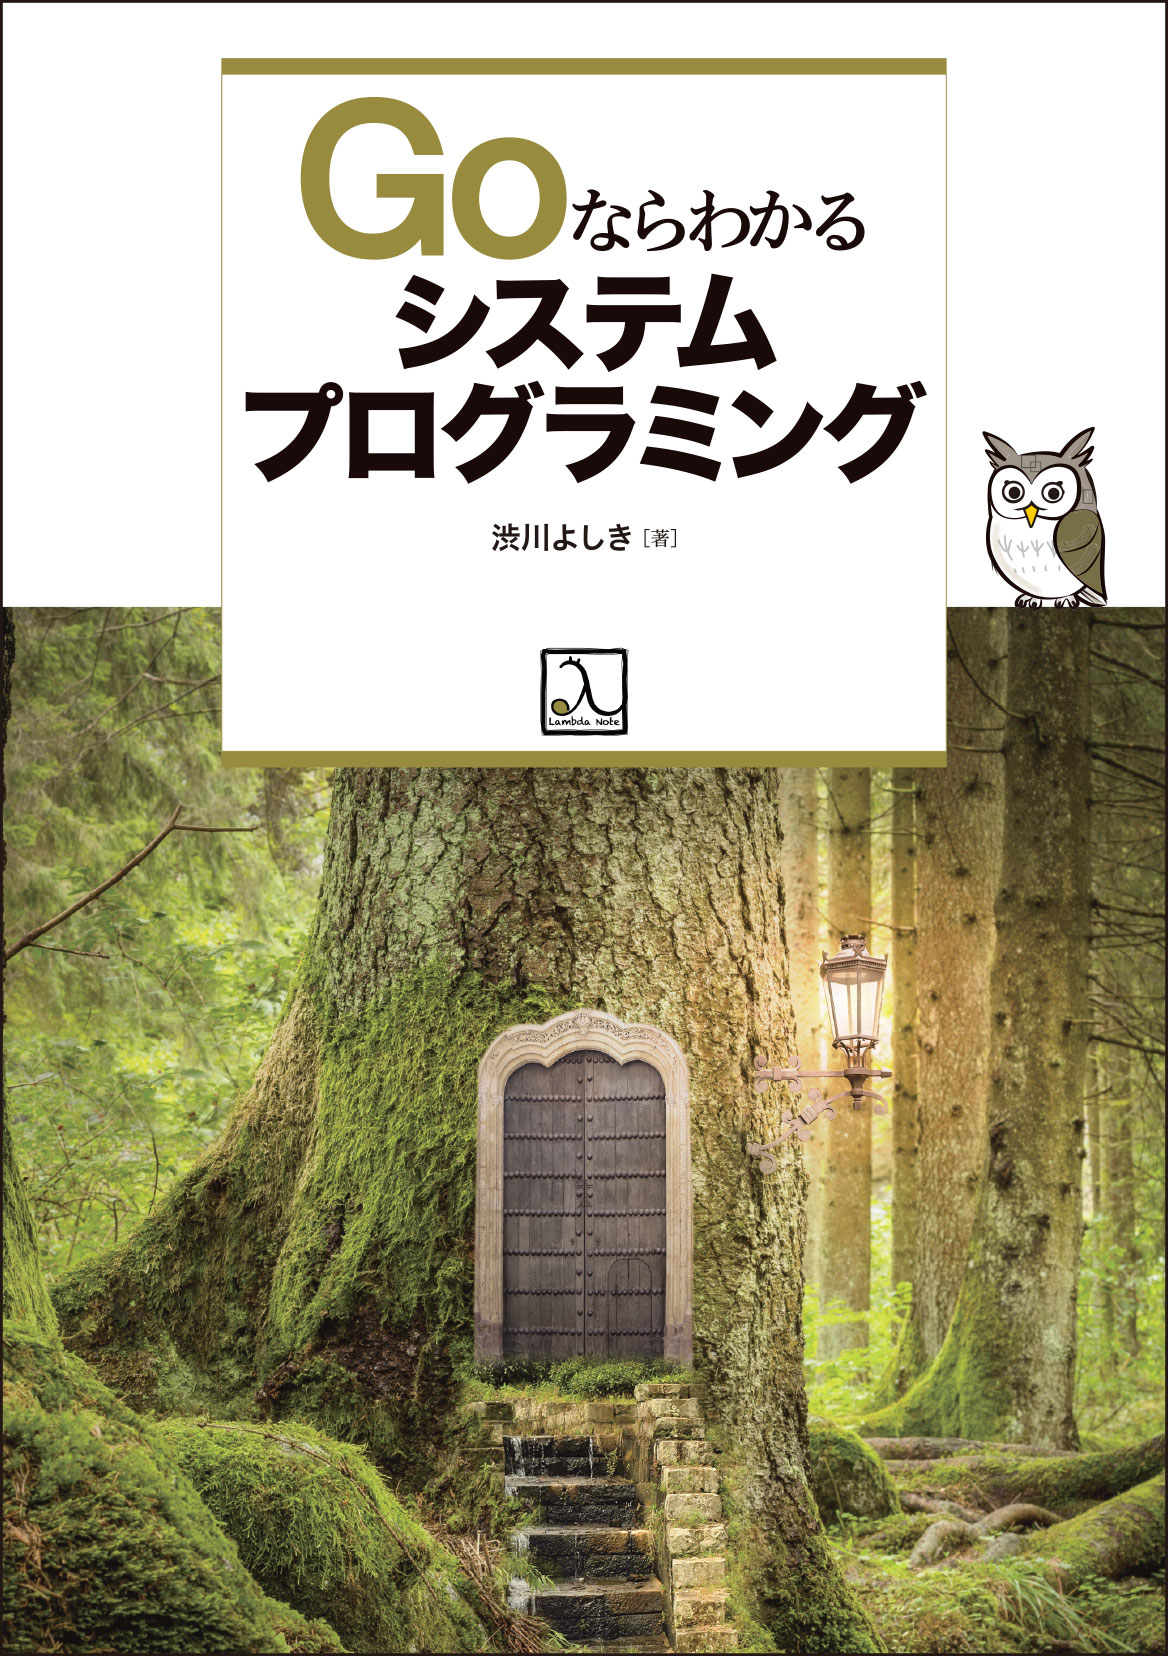
\includegraphics[width=\textwidth]{figures/progo.jpg}
    \end{column}
    \begin{column}{.5\paperwidth}
      \hspace*{2ex}[
      \vbox {\raggedright\sffamily\HUGE{12}{20}\vfill\color{white}%
      reStructuredTextでHTMLの記事が執筆されていたので、そのままSphinxでLaTeXを生成して、印刷製本用のデータを制作した
      }
      \vfill
      \vspace*{3\baselineskip}
      \hspace*{2ex}
      \vbox{\raggedright\HUGE{10}{12}\vfill\color{white}%
        渋川よしき 著\\
        A5判/360頁/本体3200円\\
        ISBN:978-4-908686-03-0\\
      }
    \end{column}
  \end{columns}
\end{frame}
\endgroup


\begin{frame}[t]{\inhibitglue Sphinxの\texttt{make latexpdf}でPDFを生成してません}
  \sffamily
    \begin{itemize}
    \item Sphinxディレクトリ下のreST原稿は、HTMLなどの生成には影響を与えず、そのままの形で完全に活用したい
   \item でも、PDFはSphinxで作りたくない。なぜなら、
    \begin{itemize}
      \item われわれは\TeX にはちょっと詳しいので
      \item 図はJPGやPNGではなくPDFを埋め込みたい
      \item クラスファイルやスタイルファイルは自前のものを使いたい(後述)
      \end{itemize}
    \item \LaTeX 制作環境下で\texttt{make}すると、
          Sphinxディレクトリ下で\texttt{make latex}して\texttt{.tex}を生成し、
          自前のルーチンでPDFが生成される、というフローを採用
    \end{itemize}

\end{frame}

\begin{frame}[t]{\inhibitglue 必要だったハック}
  \sffamily
    \begin{itemize}
      \item 1. デフォルトの\LaTeX テンプレートは使いづらい
      \item 2. 自作の\LaTeX スタイルで見た目を変えたい
      \item 3. ブロック要素内の脚注を特別扱いしたくない
      \item 4. 書籍の相互参照 ≠ ハイパーリンク
      \item 5. 整形の自由度が高い表が必要
    \end{itemize}
\end{frame}

\setbeamertemplate{background canvas}[vertical shading][bottom=white,top=yamabuki!70]
\setbeamercolor{frametitle}{bg=yamabuki, fg=black}
\setbeamercolor{structure}{fg=yamabuki}

\begin{frame}[t]{\inhibitglue 必要だったハック}
  \sffamily
    \begin{itemize}
      \onslide<1> \item 1. デフォルトの\LaTeX テンプレートは使いづらい
      \onslide<0> \item 2. 自作の\LaTeX スタイルで見た目を変えたい
      \onslide<0> \item 3. ブロック要素内の脚注を特別扱いしたくない
      \onslide<0> \item 4. 書籍の相互参照 ≠ ハイパーリンク
      \onslide<0> \item 5. 整形の自由度が高い表が必要
    \end{itemize}
\end{frame}

\begin{frame}[t,fragile=singleslide]{\inhibitglue 専用ドキュメントクラスを使いたい、\\ デフォルトのパッケージは使いたくない}
  \sffamily
  \begin{itemize}
  \item \texttt{\_template/latex.tex\_t}として、カスタマイズのテンプレートを設定することで解決できた
  \end{itemize}

  \fontsize{7.5pt}{7pt}\selectfont
  \begin{tcolorbox}
  \begin{minted}{latex}
\documentclass[a5,dvipdfmx,uplatex]{lnbook}

\usepackage{sphinx}
\usepackage{progo}
\AtBeginShipoutFirst{\special{pdf:tounicode UTF8-UTF16}}
<%= makeindex %>
\pagestyle{bookheadings}
\usepackage{hyperref}

<%= body %>
<%= atendofbody %>
<%= indices %>
<%= printindex %>
\include{okuduke}

\end{document}
\end{minted}
\end{tcolorbox}

\end{frame}

\begin{frame}[t,fragile=singleslide]{\leavevmode\inhibitglue 「章」以外の構成要素を追加したり、\\ 構成要素の順番を変えたりしたい}
  \sffamily
  \begin{itemize}
  \item 目次どころか \texttt{\bslash{}begin\{document\}}までもが \texttt{<\%= body \%>} の部分に埋め込まれてしまうので、こう書けない!
  \end{itemize}
  \fontsize{7.5pt}{7pt}\selectfont
  \begin{tcolorbox}
  \begin{minted}[highlightcolor=nanohana, highlightlines={3-8}]{latex}
\documentclass[a5,dvipdfmx,uplatex]{lnbook}
...
%%% こう書きたい!(けど、書けない)
%%% 
%%% \begin{document}
%%% \include{tobiraura}
%%% \include{preface}
%%% \tableofcontents

<%= body %>
<%= atendofbody %>
<%= indices %>
<%= printindex %>
\include{okuduke}
\end{document}
\end{minted}
\end{tcolorbox}

\end{frame}

\begin{frame}[t,fragile=singleslide]{\inhibitglue ディレクティブを追加しました}
  \sffamily
  \fontsize{7.5pt}{7pt}\selectfont
  \begin{tcolorbox}
  \begin{minted}{python}
def frontmatter(name, arguments, options, content, lineno,
                content_offset, block_text, state, state_machine):
    return [nodes.raw(
        '',
        r"""
\include{tobiraura}
\frontmatter \setcounter{page}{3}
""",
        format='latex')]

def mainmatter(name, arguments, options, content, lineno,
               content_offset, block_text, state, state_machine):
    return [nodes.raw(
        '',
        r"""
\tableofcontents
\mainmatter
""",
        format='latex')]

def setup(app):
    app.add_directive('frontmatter', frontmatter, 1, (0, 0, 0))
    app.add_directive('mainmatter', mainmatter, 1, (0, 0, 0))

  \end{minted}
  \end{tcolorbox}

\end{frame}

\begin{frame}[t,fragile=singleslide]{\inhibitglue 自在に本を構成できるようになりました}
  \sffamily

  \fontsize{7pt}{7pt}\selectfont
  \begin{multicols}{2}
    \begin{tcolorbox}[enhanced jigsaw, breakable, break at=70mm]
      \begin{minted}{rst}
Goならわかるシステムプログラミング
==================================

.. only:: latex
   
   .. frontmatter::

.. toctree::
   :maxdepth: 2

   preface

.. only:: latex

   .. mainmatter::

.. toctree::
   :maxdepth: 3
   :numbered:

   introduction
   iowriter
   :
   :
   container

.. only:: latex

   .. appendix::

.. toctree::
   :maxdepth: 3
   :numbered:

   appendix
   appendix_c

.. only:: latex

   .. backmatter::

.. toctree::

   afterword
    \end{minted}
  \end{tcolorbox}

\hfill 実際の\texttt{index.rst}のようす
\end{multicols}

\end{frame}


\begin{frame}[t,fragile=singleslide]{\inhibitglue 「はじめに」を「第\, 0章」にしたくない}
  \sffamily
  \begin{itemize}
  \item \texttt{\bslash{}chapter\{はじめに\}}になる見出しと、\texttt{\bslash{}chapter*\{はじめに\}}になる見出しとを、\\ \texttt{.rst}ファイル内で切り換えることは無理っぽい
  \item しかたがないので、Sphinxが生成した\texttt{.tex}をスクリプトで後処理してから、up\LaTeX でPDF生成
  \end{itemize}
  \fontsize{8pt}{8pt}\selectfont
  \begin{tcolorbox}
    \begin{minted}{basemake}
tex:
    cd ../; make latex
    cp ../_build/latex/Go.tex book.tex
    gosh script/post-sphinx-latex.scm      
    \end{minted}
  \end{tcolorbox}
  \hfill 実際のMakefileのようす
    
\end{frame}


\setbeamertemplate{background canvas}[vertical shading][bottom=white,top=matsuba!40]
\setbeamercolor{frametitle}{bg=matsuba, fg=white}
\setbeamercolor{structure}{fg=matsuba}

\begin{frame}[t]{\inhibitglue 必要だったハック}
  \sffamily
    \begin{itemize}
      \onslide<0> \item 1. デフォルトの\LaTeX テンプレートは使いづらい
      \onslide<1> \item 2. 自作の\LaTeX スタイルで見た目を変えたい
      \onslide<0> \item 3. ブロック要素内の脚注を特別扱いしたくない
      \onslide<0> \item 4. 書籍の相互参照 ≠ ハイパーリンク
      \onslide<0> \item 5. 整形の自由度が高い表が必要
    \end{itemize}
\end{frame}

\begin{frame}[t,fragile=singleslide]{\inhibitglue 例:コード片と実行画面を区別したい}
  \sffamily
  \begin{itemize}
  \item \texttt{.. code-block::}ディレクティブは、\LaTeX{}の\texttt{sphinxVerbatim}環境内のコンテンツへと一律に変換される
  \item つまり、PDFでの見た目をスタイルでスイッチできない
    (HTMLでは\texttt{:class:}オプションで実現可能)
  \end{itemize}

  \begin{center}
    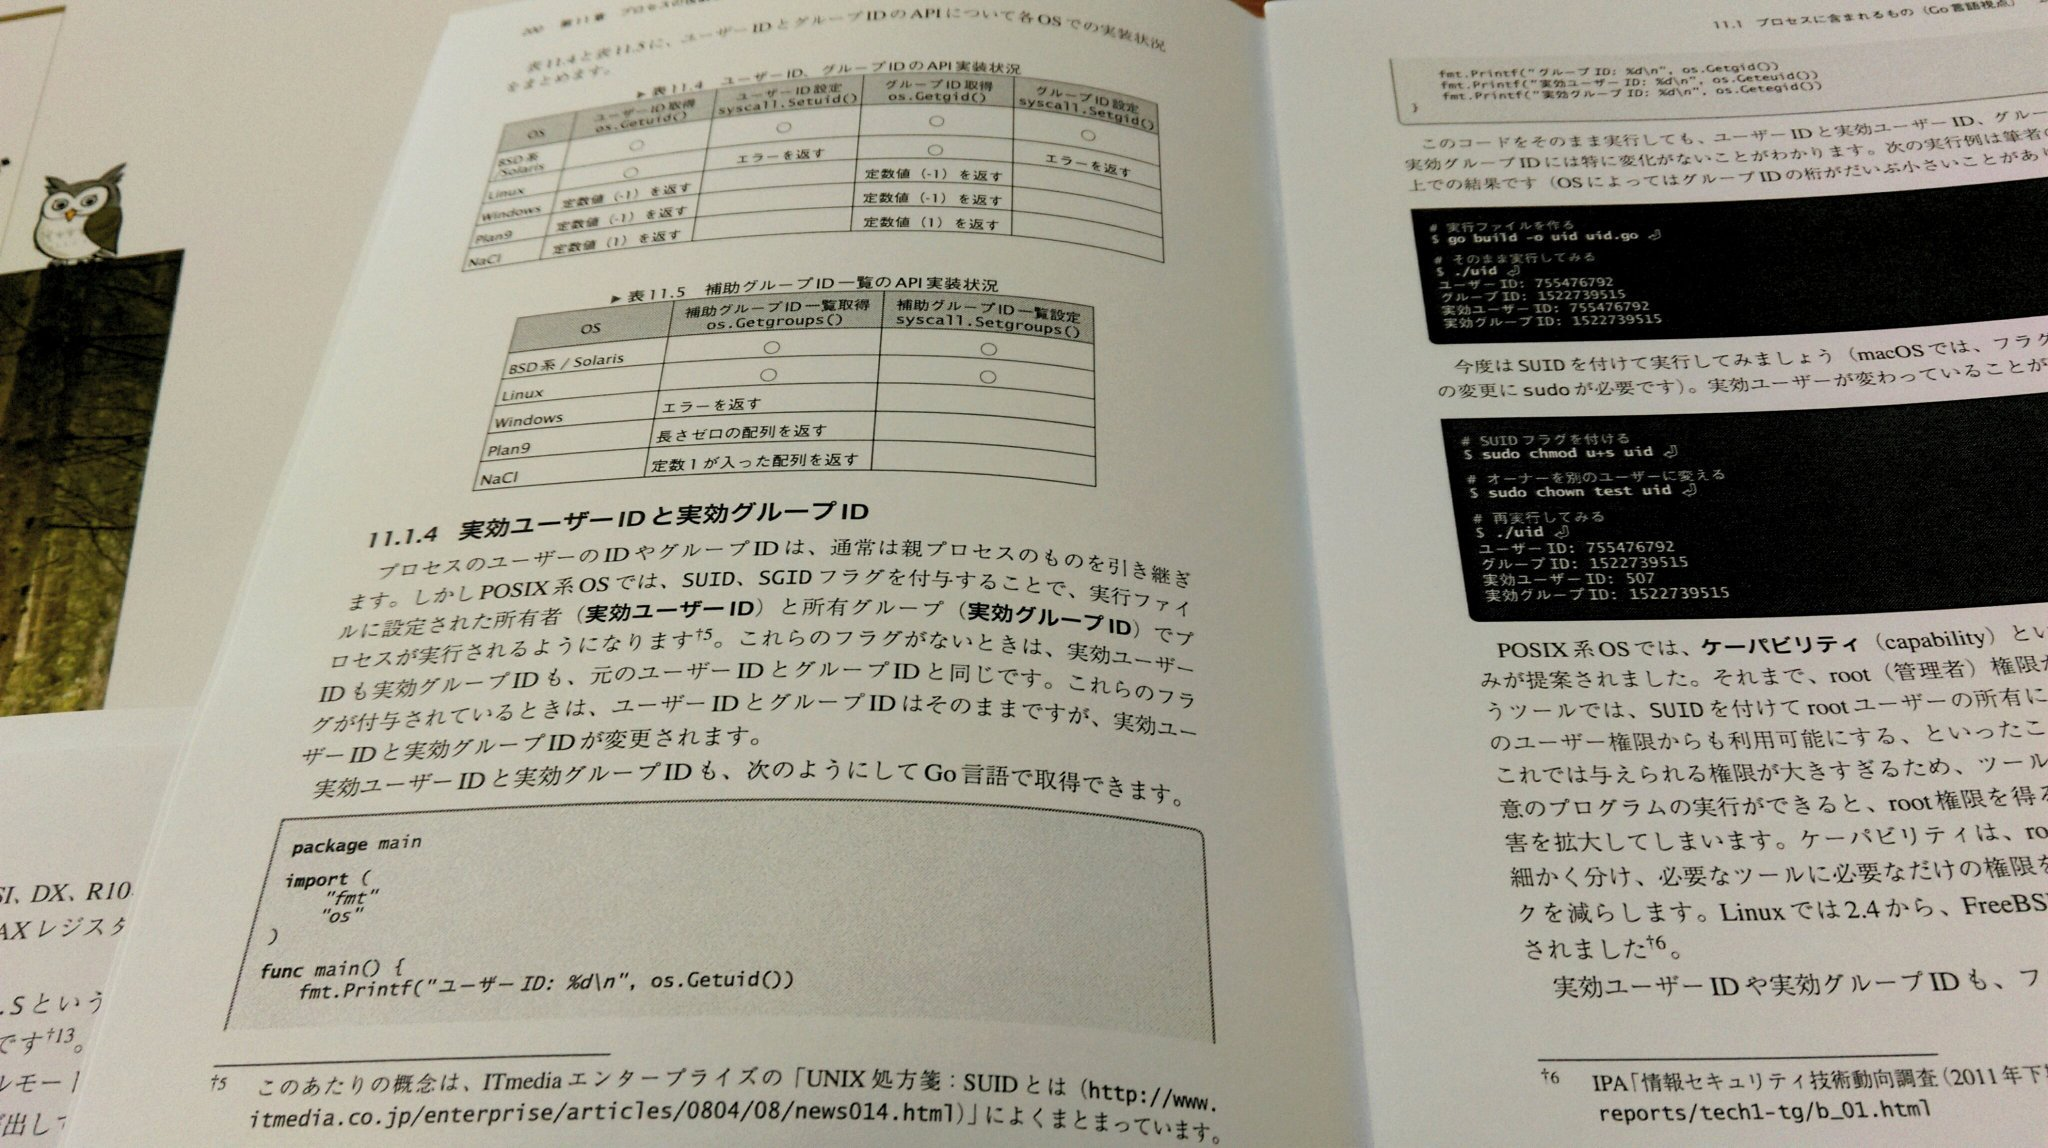
\includegraphics[width=.5\textwidth]{figures/codeenv.jpg}
  \end{center}

\end{frame}

\begin{frame}[t,fragile=singleslide]{\inhibitglue 好きな環境でラップできるようにしよう}
  \sffamily
  \begin{itemize}
  \item \texttt{code-block}の改造はつらいので \TeX でカバー
  \end{itemize}

  \fontsize{7pt}{7pt}\selectfont
  \begin{tcolorbox}
  \begin{minted}{rest}
.. customenv:: execquote

   .. code-block:: sh
   
      # apt-get install strace ⏎
  \end{minted}
  \end{tcolorbox}
  ↓ \texttt{make latex}
  \begin{tcolorbox}
  \begin{minted}[highlightcolor=nanohana, highlightlines={1,9}]{latex}
\begin{customadmonition}{execquote}

\def\sphinxLiteralBlockLabel{\label{\detokenize{systemcall:id66}}
\begin{sphinxVerbatim}[commandchars=\\\{\}]
\PYG{c+c1}{\PYGZsh{} \color{white}apt\PYGZhy{}get install strace \crmark{}}
\end{sphinxVerbatim}
\let\sphinxVerbatimTitle\empty
\let\sphinxLiteralBlockLabel\empty
\end{customadmonition}
  \end{minted}
  \end{tcolorbox}
\end{frame}


\begin{frame}[t,fragile=singleslide]{\inhibitglue issueを出した}
  \sffamily
  \begin{itemize}
  \item \texttt{.rst}内でこんな入れ子を書くのは筋悪
  \item \LaTeX{}出力で\texttt{:class:}オプションの値が捨てられてるけど、この値を環境名にしてディレクティブの出力がラップされてくれれば、\texttt{.sty}でユーザがスタイルを指定できる
    \begin{itemize}
    \item HTML出力だと\texttt{<div>}の\texttt{class}値になるのでCSSでスタイル付けできる、という話と同じです
    \end{itemize}
  \item \leavevmode\inhibitglue 「LaTeX representation for :class: (of like `..code-block::` or `..note::`) \#4010」\\
    \footnotesize\url{https://github.com/sphinx-doc/sphinx/issues/4010}
  \end{itemize}

\end{frame}


\setbeamertemplate{background canvas}[vertical shading][bottom=white,top=shozyohi!20]
\setbeamercolor{frametitle}{bg=shozyohi, fg=white}
\setbeamercolor{structure}{fg=shozyohi}

\begin{frame}[t]{\inhibitglue 必要だったハック}
  \sffamily
    \begin{itemize}
      \onslide<0> \item 1. デフォルトの\LaTeX テンプレートは使いづらい
      \onslide<0> \item 2. 自作の\LaTeX スタイルで見た目を変えたい
      \onslide<1> \item 3. ブロック要素内の脚注を特別扱いしたくない
      \onslide<0> \item 4. 書籍の相互参照 ≠ ハイパーリンク
      \onslide<0> \item 5. 整形の自由度が高い表が必要
    \end{itemize}
\end{frame}

\begin{frame}[t,fragile=singleslide]{\inhibitglue \LaTeX{}の脚注は透過的にうまく扱えない}
  \sffamily
  \begin{itemize}
  \item Sphinxでも苦労のあとが見える(\texttt{footnotehyper-sphinx.sty})
  \item Sphinx提供のスタイル以外を使う場合、それが仇になる
  \end{itemize}

  \fontsize{7pt}{7pt}\selectfont
  \begin{tcolorbox}
  \begin{minted}{python}
def visit_collected_footnote(self, node):
    # type: (nodes.Node) -> None
    self.in_footnote += 1
    if 'footnotetext' in node:
        self.body.append('%%\n\\begin{footnotetext}[%s]'
                         '\\sphinxAtStartFootnote\n' % node['number'])
    else:
        if self.in_parsed_literal:
            self.body.append('\\begin{footnote}[%s]' % node['number'])
        else:
            self.body.append('%%\n\\begin{footnote}[%s]' % node['number'])
        self.body.append('\\sphinxAtStartFootnote\n')
  \end{minted}
  \end{tcolorbox}
  \hfill \texttt{writers/latex.py} のようす
\end{frame}

\begin{frame}[t,fragile=singleslide]{\inhibitglue \TeX{}のふつうの脚注に戻しました}
  \sffamily
  \fontsize{8pt}{8pt}\selectfont
  \begin{tcolorbox}
  \begin{minted}{python}
def visit_collected_footnote(self, node):
    # type: (nodes.Node) -> None
    self.in_footnote += 1
    if 'footnotetext' in node:
        self.body.append('\\footnotetext{')
    else:
        if self.in_parsed_literal:
            self.body.append('\\footnote{')
        else:
            self.body.append('\\footnote{')

def depart_collected_footnote(self, node):
    # type: (nodes.Node) -> None
    if 'footnotetext' in node:
        self.body.append('}\\ignorespaces ')
    else:
        if self.in_parsed_literal:
            self.body.append('}')
        else:
            self.body.append('}')
    self.in_footnote -= 1

  \end{minted}
  \end{tcolorbox}
\end{frame}


\setbeamertemplate{background canvas}[vertical shading][bottom=white,top=asagi!30]
\setbeamercolor{frametitle}{bg=asagi, fg=black}
\setbeamercolor{structure}{fg=asagi}

\begin{frame}[t]{\inhibitglue 必要だったハック}
  \sffamily
    \begin{itemize}
      \onslide<0> \item 1. デフォルトの\LaTeX テンプレートは使いづらい
      \onslide<0> \item 2. 自作の\LaTeX スタイルで見た目を変えたい
      \onslide<0> \item 3. ブロック要素内の脚注を特別扱いしたくない
      \onslide<1> \item 4. 書籍の相互参照 ≠ ハイパーリンク
      \onslide<0> \item 5. 整形の自由度が高い表が必要
    \end{itemize}
\end{frame}

\begin{frame}[t,fragile=singleslide]{\inhibitglue 人間が参照先を目で探すための文字列}
  \sffamily
  \begin{itemize}
    \item \texttt{:doc:}や\texttt{:ref:}だと、章や節のタイトルしか出力しない
    \item 人間が参照先にたどり着くためには、章や節の「番号」のほうが重要だったりする
    \item かといって、\texttt{:numref:}を使うためにラベルを追加するのは面倒
  \end{itemize}
\end{frame}

\begin{frame}[t,fragile=singleslide]{\inhibitglue 独自に\texttt{:numdoc:}ロールを用意しました}
  \fontsize{7pt}{7pt}\selectfont
  \begin{tcolorbox}
  \begin{minted}{python}
def numdoc_role(name, rawtext, text, lineno, inliner, options={}, 
                content=[]):
    :
    pnode = nodes.inline(rawtext, title, classes=['xref','doc'])
    pnode['reftarget'] = target
    return [pnode], []

def visit_inline(self, node):
    classes = node.get('classes', [])
    if classes in [['menuselection'], ['guilabel']]:
        :
    elif classes in [['xref','doc']] and not self.in_title:
        self.body.append(ur'第\DUrole{%s}{' % ','.join(classes))
        self.context.append(u'}章')
    elif classes and not self.in_title:
        :
  \end{minted}
  \end{tcolorbox}

  \sffamily\footnotesize
  \begin{itemize}
    \item いにしえの互換性を維持するための機能が\texttt{sphinx.sty}にあったので、それを利用できた
  \end{itemize}

  \fontsize{7pt}{7pt}\selectfont
  \begin{tcolorbox}
  \begin{minted}{latex}
\expandafter\def\csname DUrole\detokenize{xref,doc}\expandafter\endcsname
  \expandafter{\csname ref\endcsname}
\providecommand*{\DUrole}[2]{%
    :
  \end{minted}
  \end{tcolorbox}
\end{frame}

\begin{frame}[t,fragile=singleslide]{\inhibitglue 相互参照UIの落としどころ難しい}
  \sffamily\small
  \begin{itemize}
    \item \texttt{:numdoc:}と\texttt{:doc:}を併記するのは、ちょっといけてない
    \item \texttt{:numref:}と\texttt{:ref:}も併記するしかないし、まあいいかな
    \item そもそも現在のSphinxでは参照アンカーをすべてSphinx側で事前に解決し、その結果を\texttt{\bslash{}hyperref}のオプション引数に埋め込んでしまう。でも、節番号の相互参照のような「\LaTeX{}が得意なこと」は、\LaTeX{}にやらせたい
    \begin{itemize}
      \item \LaTeX{}には採番機能があるけど、HTMLやEPUBに対応するには上位で採番機能が必要なんだよな
      \item \LaTeX{}にしても、章や節のタイトル再利用は大変なので、どうがんばっても痒みは残りそうではある…
    \end{itemize}
    \item HTMLやEPUBでは無意味だけど、PDFでは\LaTeX{}の「ページ参照」が使いたい
  \end{itemize}
\end{frame}

\begin{frame}[t,fragile=singleslide]{\inhibitglue ページ参照といえば、索引}
  \sffamily
  \begin{itemize}
    \item 索引のアンカーは、「項目が出現するセクション」ではなく、「項目が出現するページ」に必要
    \item 必然的に、\texttt{.. index::}ディレクティブが使えない……
  \end{itemize}
\end{frame}

\begin{frame}[t,fragile]{\inhibitglue 独自に\texttt{:tex:}ロールを用意しました}
  \setbeamercovered{invisible}
  \fontsize{7pt}{7pt}\selectfont  
  \begin{tcolorbox}
  \begin{minted}{python}
def tex_role(name, rawtext, text, lineno, inliner, options={}, content=[]):
    text = utils.unescape(text, restore_backslashes=True)
    has_explicit, texsnipet, target = split_explicit_title(text)
    pnode = nodes.raw(rawtext, texsnipet, format='latex')
    return [pnode], []

def setup(app):
    app.add_role('tex', tex_role)
  \end{minted}
  \end{tcolorbox}

  \sffamily\small
  \begin{itemize}
    \item 局所的な\TeX{}ソースの埋め込みによるスタイル指定にも使えて、やりたい放題!\pause
    \item でも、原稿がこうなるの、いやですよね?
  \end{itemize}

  \fontsize{7pt}{7pt}\selectfont
  \begin{tcolorbox}
  \begin{Verbatim}[breaklines,breakanywhere,
breakautoindent=false,
breaksymbolindentleft=0pt,
breaksymbolsepleft=0pt,
breaksymbolindentright=0pt,
breaksymbolsepright=0pt]
物理的なストレージと対応しない、仮想的なファイルシステム\ :tex:`\index{ファイルシステム!仮想的な}`\ もあります。
たとえば、Unix系のシステムにおける\ ``/proc``\ :tex:`\index{proc@\texttt{/proc}}`\ は仮想的なファイルシステムの一例です。
  \end{Verbatim}
  \end{tcolorbox}
\end{frame}


\begin{frame}[t,fragile=singleslide]{\inhibitglue 索引専用の\, Gitブランチを使う}
  \sffamily
  \begin{itemize}
  \item 索引タグは、編集者だけが煩わされればよい
  \item indexingブランチにmasterからcherry-pickしてmakeしたものを最終入稿データとする
  \item 索引が組まれた\LaTeX{}用ファイルのみをmasterにコピーするという運用もありえる
  \end{itemize}

  \begin{center}
    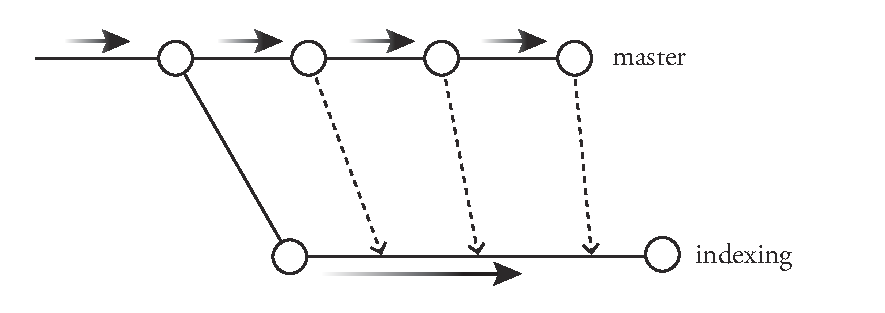
\includegraphics[width=.8\textwidth]{figures/indexing.pdf}
  \end{center}
  \fontsize{7pt}{7pt}\selectfont
  \hfill \url{https://www.slideshare.net/k16shikano/imybp-light}より
\end{frame}

\setbeamertemplate{background canvas}[vertical shading][bottom=white,top=hiwa!50]
\setbeamercolor{frametitle}{bg=hiwa, fg=black}
\setbeamercolor{structure}{fg=hiwa}

\begin{frame}[t]{\inhibitglue 必要だったハック}
  \sffamily
    \begin{itemize}
      \onslide<0> \item 1. デフォルトの\LaTeX テンプレートは使いづらい
      \onslide<0> \item 2. 自作の\LaTeX スタイルで見た目を変えたい
      \onslide<0> \item 3. ブロック要素内の脚注を特別扱いしたくない
      \onslide<0> \item 4. 書籍の相互参照 ≠ ハイパーリンク
      \onslide<1> \item 5. 整形の自由度が高い表が必要
    \end{itemize}
\end{frame}


\begin{frame}[t]{\inhibitglue \LaTeX{}の表は自動できれいには組めない}
  \setbeamercovered{invisible}
  \sffamily
  \begin{itemize}
  \item Sphinxでは、表スタイルの自動解決を\LaTeX{}(tabularyパッケージ)にやらせる戦術
  \item しかし、列幅や列のスタイルを\LaTeX{}側で完全に自動で「いい感じ」にするのは無理
  \item そのため、個人的には、各セルを \texttt{\bslash{}multicolumn} 化して完全に独立制御する戦術をとっている
  \item せめて colspec を\texttt{.rst}で指定できれば……
  \end{itemize}
\pause
  \begin{center}
    
\includegraphics[width=.5\textwidth]{figures/tkomiya-tweet.png}
  \end{center}
  \fontsize{7pt}{7pt}\selectfont
  \hfill \url{https://twitter.com/tk0miya/status/909614165852954627}

\end{frame}

\setbeamertemplate{background canvas}[vertical shading][bottom=white,top=ginnezumi!20]
\setbeamercolor{frametitle}{bg=ginnezumi, fg=white}
\setbeamercolor{structure}{fg=ginnezumi}

\begin{frame}[t]{\inhibitglue まとめ}
  \setbeamercovered{invisible}
  \sffamily
  \begin{itemize}
    \item Sphinxで困ったら日本語でツイートすればいい \pause
    \item ある程度リッチな紙の本をテキストからmakeいっぱつで作るには、所与のフォーマットと拡張のための機能がSphinxくらい充実していても、手をかけないといけない部分がけっこうある
    \item ラムダノート株式会社は出版を中心として技術文書まわりのお手伝いをいろいろする会社です
    \begin{itemize}
      \item \url{https://lambdanote.com}
    \end{itemize}
  \end{itemize}
  \begin{center}
    
\includegraphics[width=.5\textwidth]{figures/main-logo.pdf}
  \end{center}
\end{frame}

\end{document}
